
% Copyright 2020 by Robert Hildebrand
%This work is licensed under a
%Creative Commons Attribution-ShareAlike 4.0 International License (CC BY-SA 4.0)
%See http://creativecommons.org/licenses/by-sa/4.0/

%\documentclass[../main/main.tex]{subfiles}
%
%%%%%%%%%%
%\begin{document}
%%%%%%%%%

\titlepic{
%	\begin{center}
%	\begin{tabular}{ccccc}
%	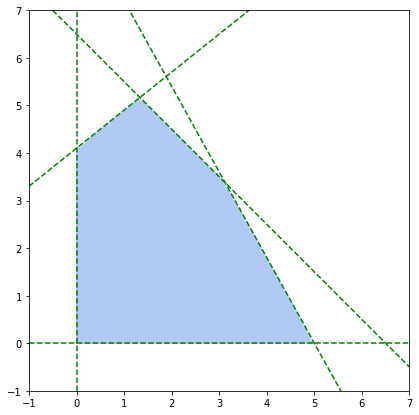
\includegraphics[scale = 0.3]{LP-feasible-region}  & \quad & 
%	 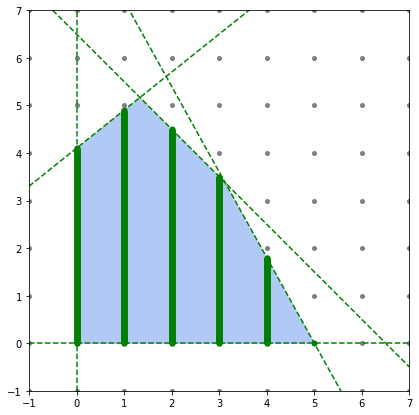
\includegraphics[scale = 0.3]{MIP-feasible-region} & \quad &
%	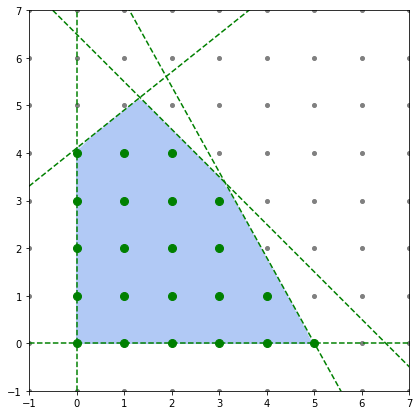
\includegraphics[scale = 0.3]{IP-feasible-region}%% \\
%	%% LP && MIP && IP\\
%	%% \\
%	%% $Ax \leq b$ & &$Ax \leq b$ && $Ax \leq b$\\
%	%% & &$x_1 \in \Z$ & &$x_1, x_2 \in \Z$
%	\end{tabular}
%	\end{center}\nopagebreak
%        \begin{center}
%          
\includegraphics[width=\linewidth]{open-optimization-common/logos/logo-open-optimization-oer-wide}
%        \end{center}
         \hyperlink{toc}{Table of Contents}
}
\maketitle

%%% Copyright page
\thispagestyle{empty}
%%\includegraphics[scale = 0.65]{creative-commons-statement}

%\begin{tabular}{p{.3\linewidth}@{\qquad}p{.55\linewidth}}
%  \begin{minipage}[c]{\linewidth}
%    \centering\Huge\ccCopy
%  \end{minipage}
%  & \begin{minipage}[c]{\linewidth}
%    Copyright 2019 by the contributors listed on the title page.
%  \end{minipage}
%  \\\\[2ex]
%  \begin{minipage}[c]{\linewidth}
%    \doclicenseImage[imagewidth=\linewidth]%
%  \end{minipage}
%  & \begin{minipage}[c]{\linewidth}%
%    \doclicenseLongText\par\vspace{-1ex}
%    \raggedleft
%    \url{https://creativecommons.org/}
%  \end{minipage}
%  \\\\[2ex]
%  \begin{minipage}[c]{\linewidth}
%    \centering\Huge\ccShareAlike 
%  \end{minipage}
%  & \begin{minipage}[c]{\linewidth}
%    This license allows everyone to remix, tweak, and build upon this work, even for
%    commercial purposes, \dots\ as long as they license their new
%    creations under identical terms \dots
%  \end{minipage}
%  \\\\[2ex]
%  \begin{minipage}[c]{\linewidth}
%    \centering\Huge\ccAttribution
%  \end{minipage}
%  & \begin{minipage}[c]{\linewidth}
%    \dots\ and if they credit the copyright holders.
%  \end{minipage}
%  \\\\[2ex]
%    \begin{minipage}[c]{\linewidth}
%    \includegraphics[width=\linewidth]{open-optimization-common/logos/Global_Open_Educational_Resources_Logo.svg}\footnotemark
%  \end{minipage}
%  & \begin{minipage}[c]{\linewidth}
%    This work aligns with the mission of UNESCO Open Educational
%    Resources.\par\vspace{1ex}
%    \raggedleft
%    \url{https://en.unesco.org/themes/building-knowledge-societies/oer}
%  \end{minipage}
%  \\\\[2ex]
%  \begin{minipage}[c]{\linewidth}
%    \centering\LARGE\LaTeX
%  \end{minipage}
%  & \begin{minipage}[c]{\linewidth}
%    The source code of this book is available.\par\vspace{1ex}
%    \raggedleft
%    \url{https://github.com/open-optimization/}
%  \end{minipage}
%\end{tabular}

%\begin{center}
%\end{center}
%\footnotetext{\url{https://en.wikipedia.org/wiki/Open_educational_resources\#/media/File:Global_Open_Educational_Resources_Logo.svg}}

\newpage

%
%%%%%%%%%%
%\end{document}
%%%%%%%%%%
%%% Local Variables:
%%% mode: latex
%%% TeX-master: "../open-optimization/open-optimization"
%%% End:
